\section{Analysis Metric 4: Unique Hexadecimal Values}
\label{sec:analysisHex}

The fourth metric we analyzed is the count of unique hexadecimal values found across all plain-text files of an \ac{npm} package version.
It was motivated by the obfuscation technique used in Attacks~B (\cref{sec:attackB}) and~D (\cref{sec:attackD}),
which encodes variable and function names as hexadecimal tokens to hide malicious behavior from static analysis,
introducing obfuscated code that makes extensive use of such tokens.
The intuition is that legitimate packages rarely encode their identifiers in this way,
so a sudden increase in this count in a new version would constitute an anomalous signal worth investigating.

\subsection{Analysis of the Goodware Dataset}
\label{subsec:goodwareHex}

\begin{figure}[htb]
    \centering
    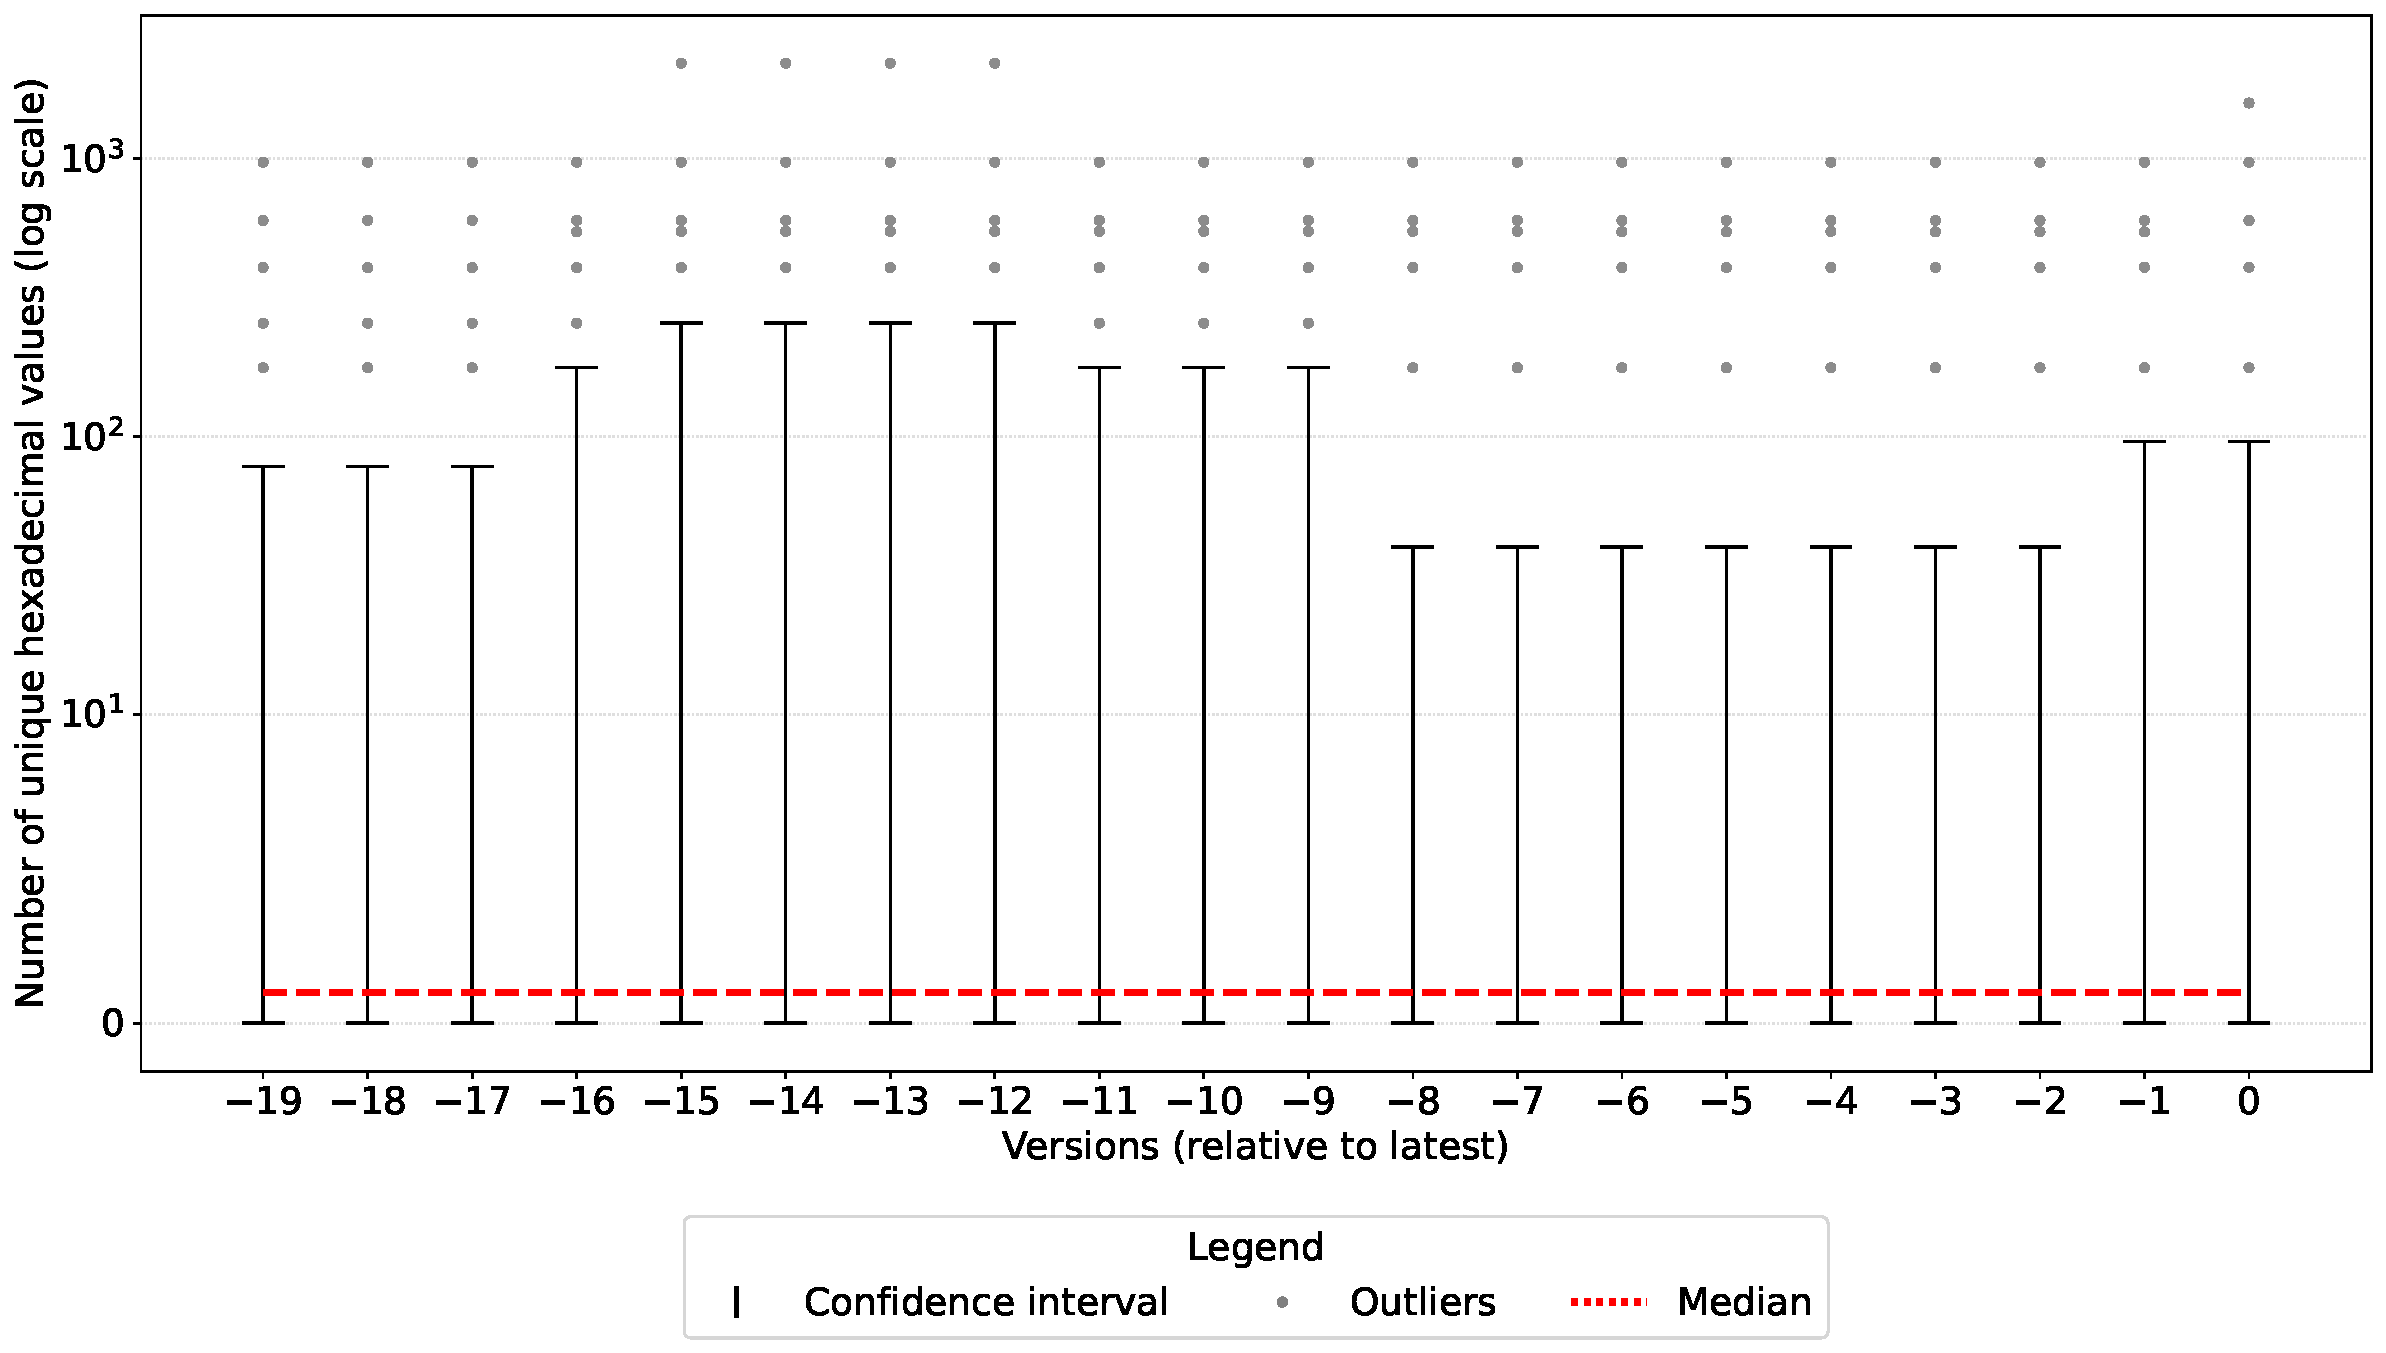
\includegraphics[width=\textwidth]{metrics/hex/hex_plot1.pdf}
    \caption{Unique Hexadecimal Values Metric: Package Trend in Goodware Dataset.}
    \label{fig:fig1Hex}
\end{figure}

The goodware dataset provides, for each of the 629 packages,
the count of unique hexadecimal values observed in their 20 analyzed versions,
as described in \cref{subsec:goodwareDataset}.
Of these, 520 have zero such values across all versions,
and carry no information for this metric; the analysis in this section is therefore
restricted to the remaining 109 packages (17.3\%),
each having at least one non-zero value in a given version.
Within this subset, the median count remains constant at 1 across all versions.
To visualize the distribution and evolutionary patterns of this metric across releases,
we used \Cref{fig:fig1Hex,fig:fig1HexIncreasing,fig:fig1HexDecreasing,fig:fig1HexStable}.
Among the considered packages, 
ten exhibit outlier or near-outlier values for at least one release and were selected for individual analysis.
The three main causes of legitimate high hexadecimal counts are 
cryptographic constants (precomputed lookup tables and algorithm parameters),
accidental inclusions, 
and build-tool-generated JavaScript files that use hexadecimal encoding for efficiency. 
Understanding these cases is essential to distinguish legitimate anomalies from malicious injections when evaluating the malware dataset.
These ten packages are highlighted in the following figures with solid colored lines, categorizing them as follows based on their observed trends:
\begin{itemize}
    \item \textbf{Increasing Trend} (\cref{fig:fig1HexIncreasing}): illustrates highlighted packages with an increasing trend over time.
    \item \textbf{Decreasing Trend} (\cref{fig:fig1HexDecreasing}): shows highlighted packages characterized by a reduction in this value.
    \item \textbf{Stable Trend} (\cref{fig:fig1HexStable}): displays highlighted packages maintaining a constant value throughout their history.
\end{itemize}

\begin{figure}[htb]
    \centering
    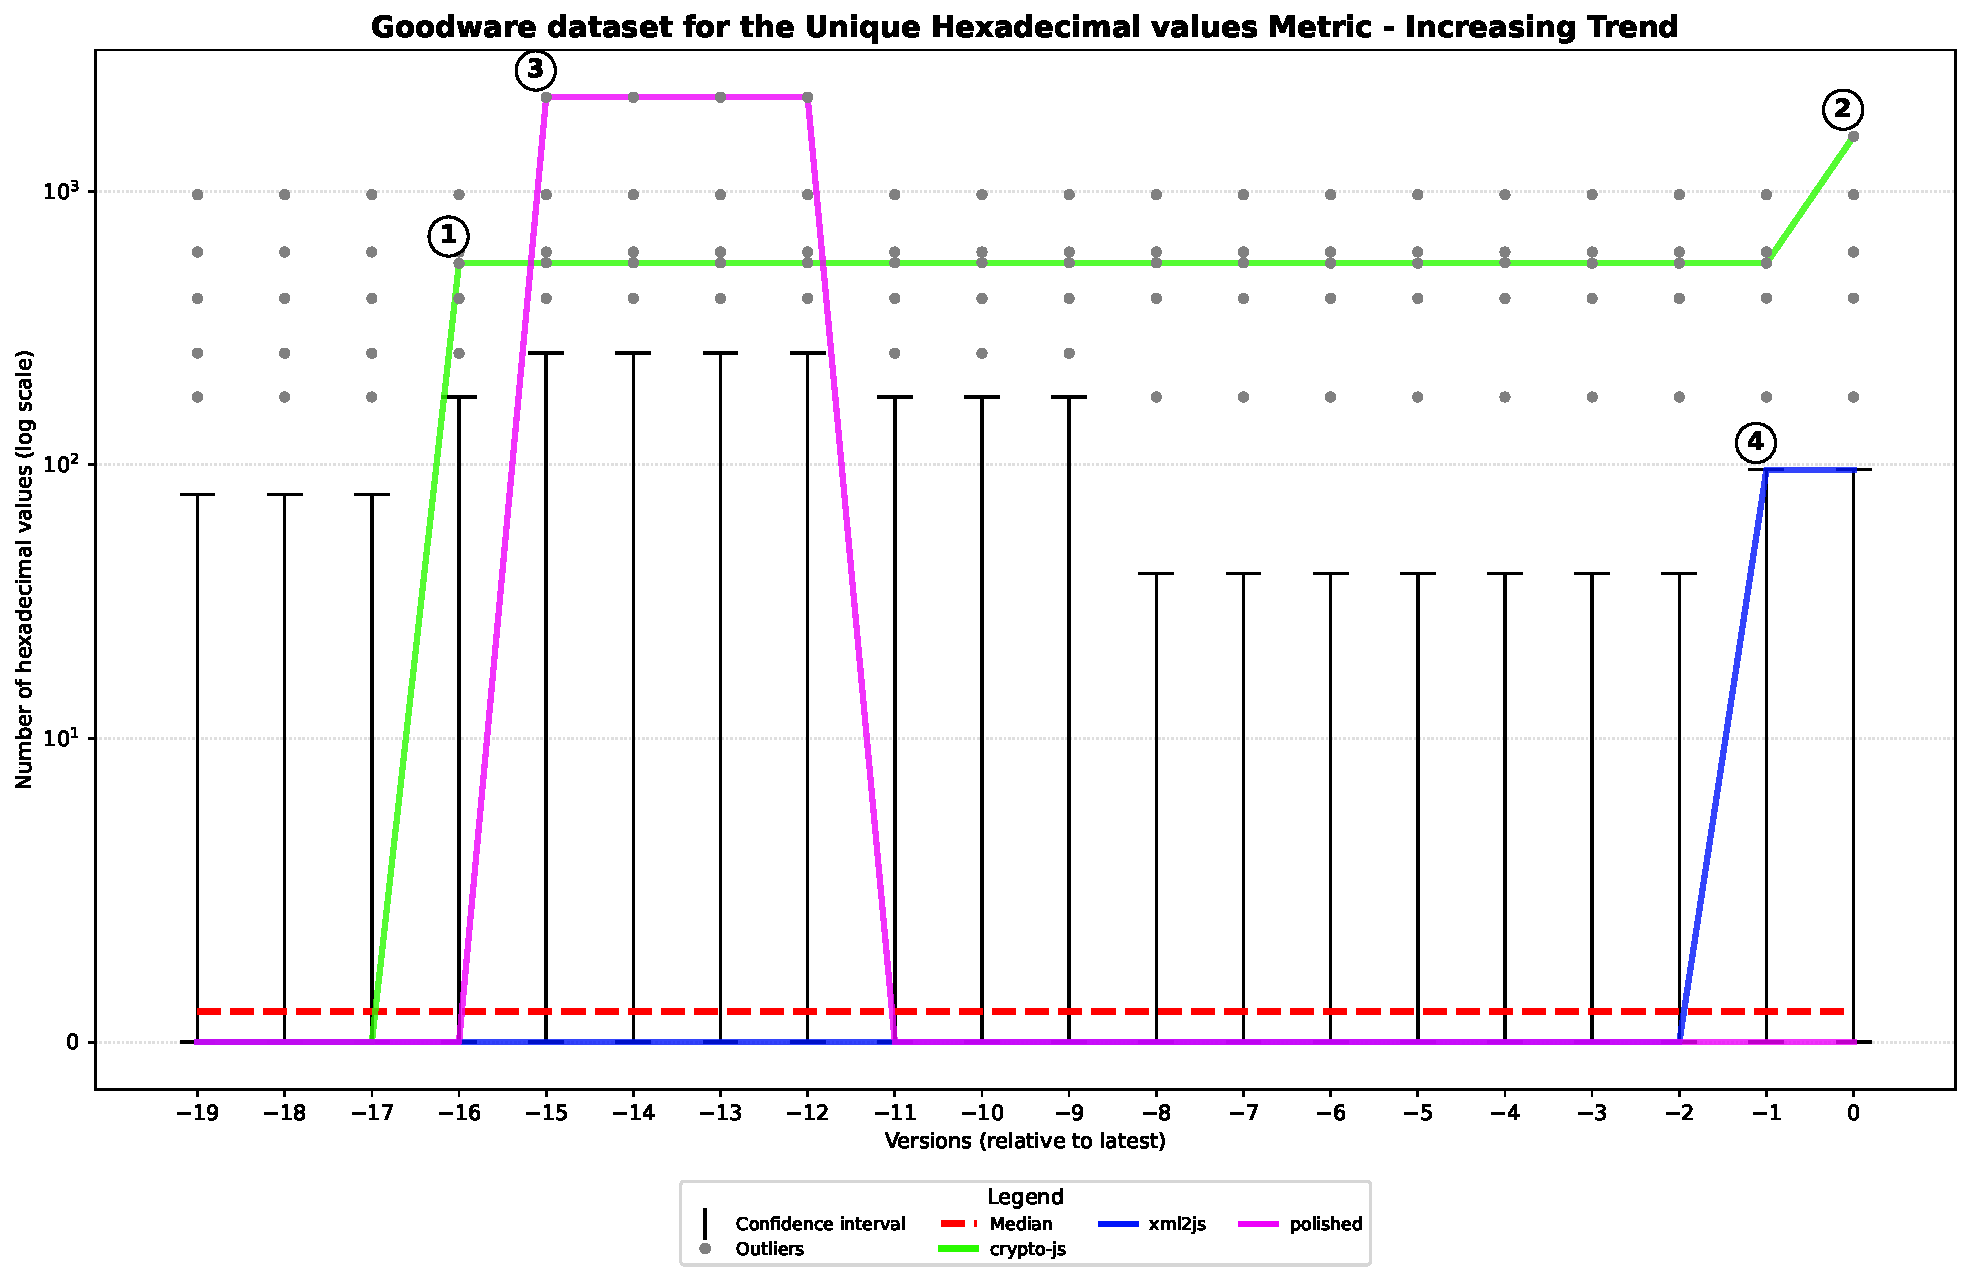
\includegraphics[width=\textwidth]{metrics/hex/hex_plot1_Increasing_Trend.pdf}
    \caption{Unique Hexadecimal Values Metric: Outliers Package Increasing Trend in Goodware Dataset.}
    \label{fig:fig1HexIncreasing}
\end{figure}

\cref{fig:fig1HexIncreasing} shows three packages that experienced a significant increase in this metric at a specific release: 
\texttt{crypto-js}, \texttt{polished}, and \texttt{xml2js}.

\textbf{crypto-js} (solid green line) is a cryptographic package that implements standard primitives, 
such as encryption algorithms and digital signatures~\cite{crypto-js}.
In its first three versions from thirteen years ago (3.1.2 to 3.1.2-2),
cryptographic constants were stored in decimal format, yielding a metric value of~0.
As shown at {\large\ding{172}} in \cref{fig:fig1HexIncreasing},
in version 3.1.2-3 the developers converted these values to hexadecimal,
aligning with standard cryptographic specification practices, such as the Secure Hash Algorithm~\cite{gallagher1995secure}.
This brought the count to 546, an outlier maintained in subsequent versions.
A further jump at {\large\ding{173}} corresponds to the introduction of the Blowfish algorithm in version 4.2.0, 
which added new hexadecimal constants and raised the count to 1,588, making it the most extreme outlier in the latest version.

\textbf{polished} (solid pink line) is a styling package for JavaScript~\cite{polished}.
As seen at {\large\ding{174}} in \cref{fig:fig1HexIncreasing}, 
it jumped from 0 to 2,208 in version 4.0.0-beta.2, the most extreme outlier for four consecutive releases.
This happened because the developers accidentally included a \texttt{.yarn} cache directory containing numerous files, including a build-tool-generated JavaScript file,
as also discussed in \Cref{subsec:goodwarePackageSize,subsec:analysisFileTypesGoodware}.
When the folder was removed in version 4.0.4~\cite{polished_release_notes}, the count returned to~0.
This is an example of an accidental anomaly traceable to a documented release note, 
distinguishable from a malicious injection because it is explained and subsequently corrected.

\begin{figure}[htbp]
    \centering
    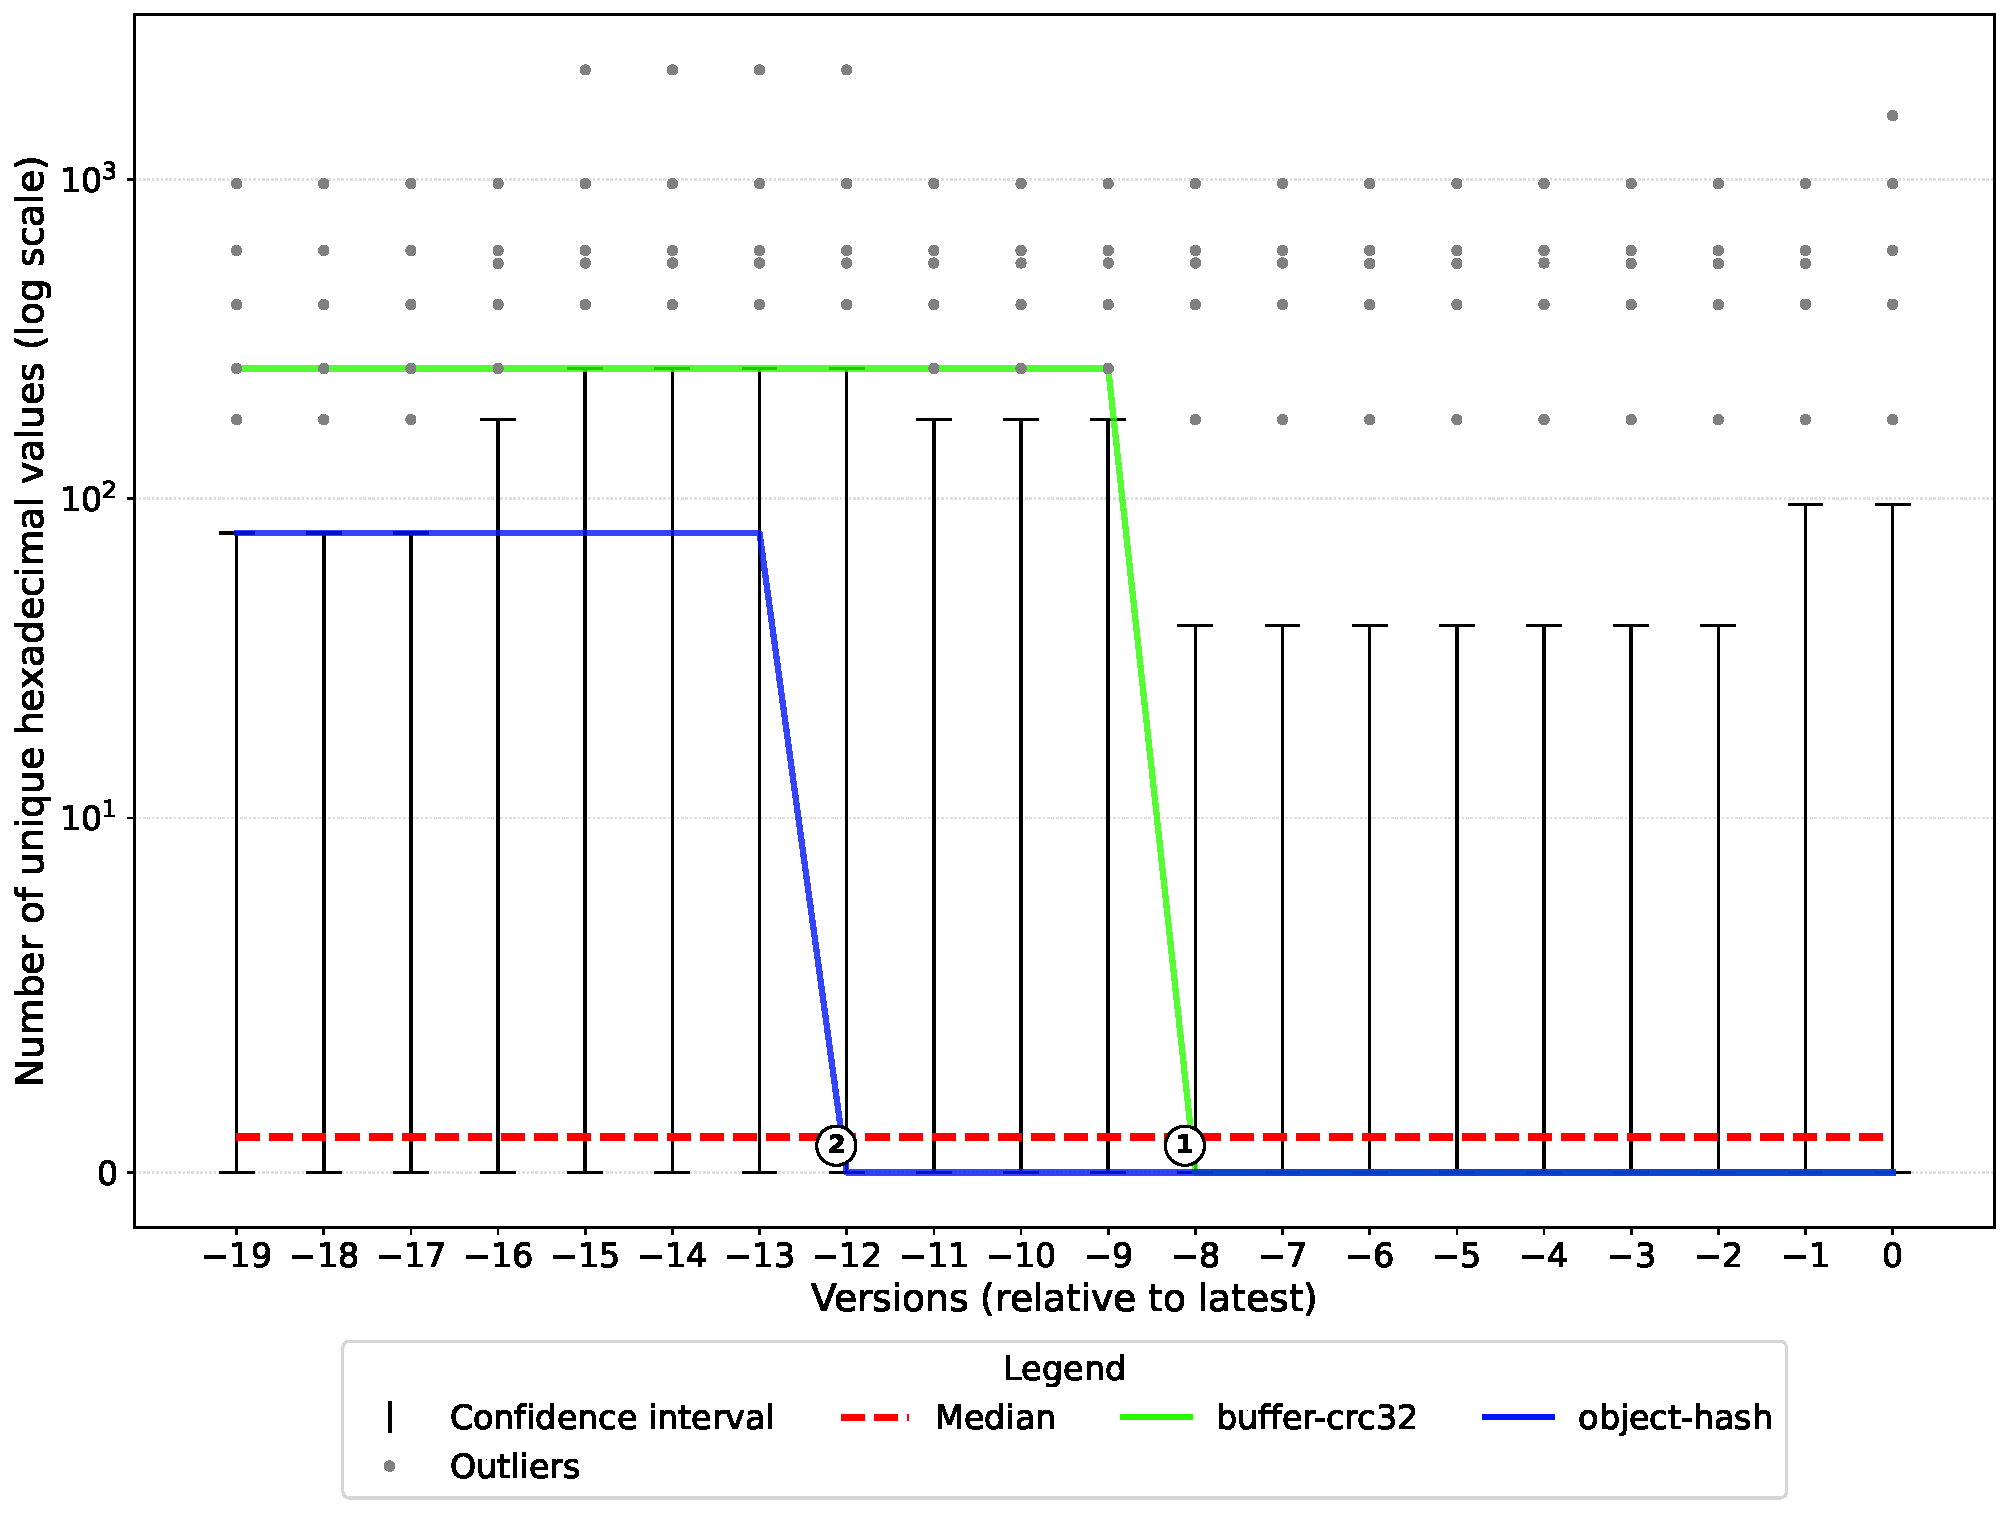
\includegraphics[width=0.76\textwidth]{metrics/hex/hex_plot1_Decreasing_Trend.pdf}
    \caption{Unique Hexadecimal Values Metric: Outliers Package Decreasing Trend in Goodware Dataset.}
    \label{fig:fig1HexDecreasing}

    \vspace{0.3cm} % Spazio verticale tra i due grafici

    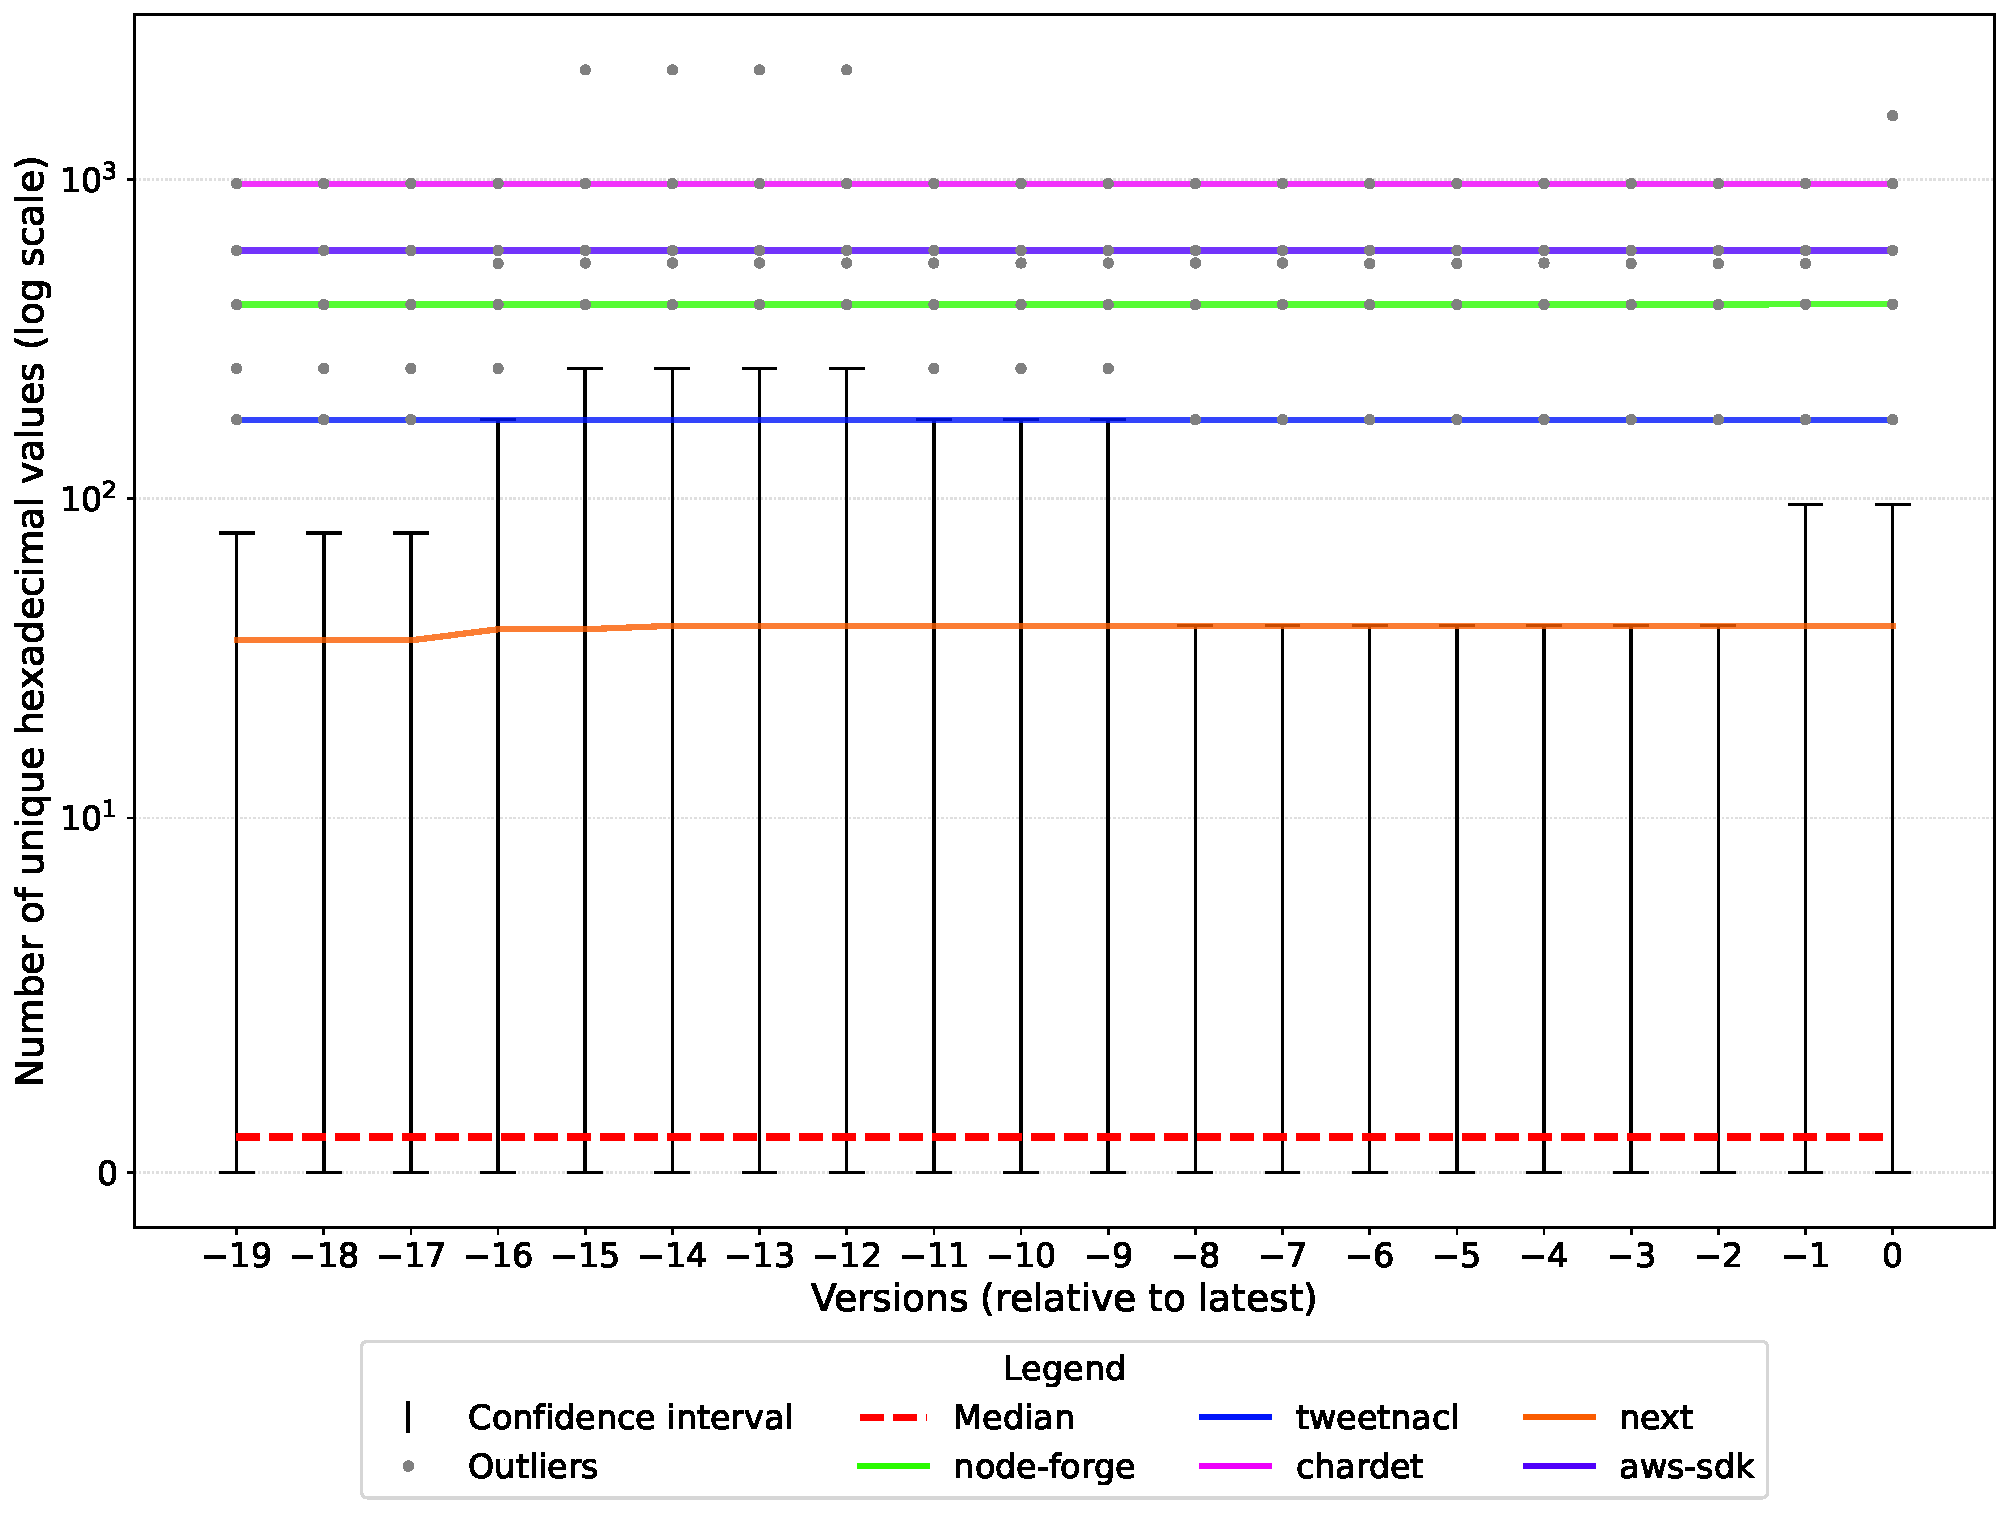
\includegraphics[width=0.76\textwidth]{metrics/hex/hex_plot1_Stable_Trend.pdf}
    \caption{Unique Hexadecimal Values Metric: Outliers Package Stable Trend in Goodware Dataset.}
    \label{fig:fig1HexStable}
\end{figure}

\textbf{xml2js} (solid blue line) went from~0 to~96 unique hexadecimal values at {\large\ding{175}} in \cref{fig:fig1HexIncreasing}.
Starting from version 0.6.1, 
the developers included a JavaScript file automatically generated from OCaml source using the \texttt{js\_of\_ocaml} compiler,
which produces output that uses such constants extensively for efficiency.
The generated file remained in the package for the subsequent version 0.6.2.

Two packages experienced a notable decrease: \texttt{buffer-crc32} and \texttt{object-hash}, as shown in \cref{fig:fig1HexDecreasing}.

\textbf{buffer-crc32} (solid green line) implements the Cyclic Redundancy Check (CRC) algorithm for data integrity checking~\cite{buffer-crc32}.
For efficiency reasons, the algorithm uses a CRC table, 
a matrix of 256 precalculated values that prevents the processor from performing complex mathematical calculations on every single byte.
Until version 0.2.13, the CRC table values were stored as hexadecimal constants.
As shown at {\large\ding{172}} in \cref{fig:fig1HexDecreasing}, 
from version 1.0.0-RC1 onward the developers switched to a build-tool-generated version of the table 
in which the values were converted to decimal for compactness.
The count therefore dropped from 256 to~0 without any change in behavior.

\textbf{object-hash} (solid blue line) is a package that generates a hash from JavaScript objects~\cite{object-hash}.
From release -19 to -17 (1.1.0 to 1.1.2),
it represented the upper limit of the confidence intervals, having 78 unique hexadecimal values, 
all located in the test file \texttt{object\_hash\_test.js}.
At {\large\ding{173}} in \cref{fig:fig1HexDecreasing}, 
starting from version 1.1.7, the test file was excluded from the published tarball for space optimization, 
as it is not essential for its functionality and not needed by end users.
The count therefore dropped to~0.

Five packages maintain stable outlier or near-outlier values across all releases.

\textbf{node-forge} and \textbf{tweetnacl} are both cryptographic packages that use hexadecimal constants as part
of their primitive implementations~\cite{node-forge, tweetnacl}, analogously to \texttt{crypto-js}.
In \cref{fig:fig1HexStable}, \texttt{node-forge} (solid green line) and \texttt{tweetnacl} (solid blue line) 
exhibit 406 and 177 unique hexadecimal values, respectively, 
qualifying as outliers in either all or the vast majority of releases.

\textbf{chardet} (solid pink line) detects character encoding using byte maps stored as 
hexadecimal constants in \texttt{/lib/encoding/sbcs.js}~\cite{chardet}, resulting in 972 values.
As shown in \cref{fig:fig1HexStable},
this makes \texttt{chardet} the extreme outlier for most releases, 
surpassed only by \texttt{polished} during its four anomalous versions and by \texttt{crypto-js} in its most recent ones.

\textbf{next} (solid orange line) and \textbf{aws-sdk} (solid purple line) 
both contain hexadecimal values in generated JavaScript files bundled in their tarballs, 
in the same manner as \texttt{polished} and \texttt{buffer-crc32}.
\texttt{next}, a React full-stack framework~\cite{next}, 
has 40 such values consistently across all releases,
representing the upper limit of the confidence intervals for versions -8 to -2, as shown in \cref{fig:fig1HexStable}.
Instead \texttt{aws-sdk}, the official package for interacting with \ac{AWS} cloud services~\cite{aws-sdk},
has 600 across all releases and is an outlier in every version.

\subsection{Comparison with the Malware Dataset}
\label{subsec:analysisHexComparisonMalware}

\textbf{Attack~A} (Malicious Windows DLL, \cref{sec:attackA}) does not introduce any new hexadecimal values,
as the malicious \ac{DLL} is binary and excluded from computation, and the \texttt{install.js} script contains no hexadecimal tokens.
As shown in \cref{fig:fig2HexAttackA}, the metric value is unchanged relative to the preceding legitimate versions, 
and the metric is not indicative for this attack.

\textbf{Attack~B} (Crypto attack, \cref{sec:attackB}) injects an obfuscated line of code into an existing \texttt{index.js} file.
The resulting count of unique hexadecimal values reaches 455.
As shown in \cref{fig:fig2HexAttackB}, this positions the malicious versions among the outliers of the goodware distribution, 
making the metric effective for detecting Attack~B.

\textbf{Attack~C} (\texttt{Shai-Hulud}~1.0, \cref{sec:attackC}) introduces a malicious file containing only one unique hexadecimal value.
As shown in \cref{fig:fig2HexAttackC}, this marginal increase leaves the compromised
releases within the confidence intervals of the goodware dataset, 
making the metric not indicative for this attack.
This outcome is consistent with the nature of the \ac{SSCA} as it does not rely on any obfuscation technique, 
but rather on the presence of clear-text malicious code.

\textbf{Attack~D} (\texttt{Shai-Hulud}~2.0, \cref{sec:attackD}) introduces an obfuscated file
using the same hexadecimal encoding technique as Attack~B.
As shown in \cref{fig:fig2HexAttackD}, the count jumps to 122,535, far exceeding the maximum outlier values observed in the goodware dataset.
The metric is clearly effective for detecting Attack~D.

\begin{figure}[htb]
    \centering
    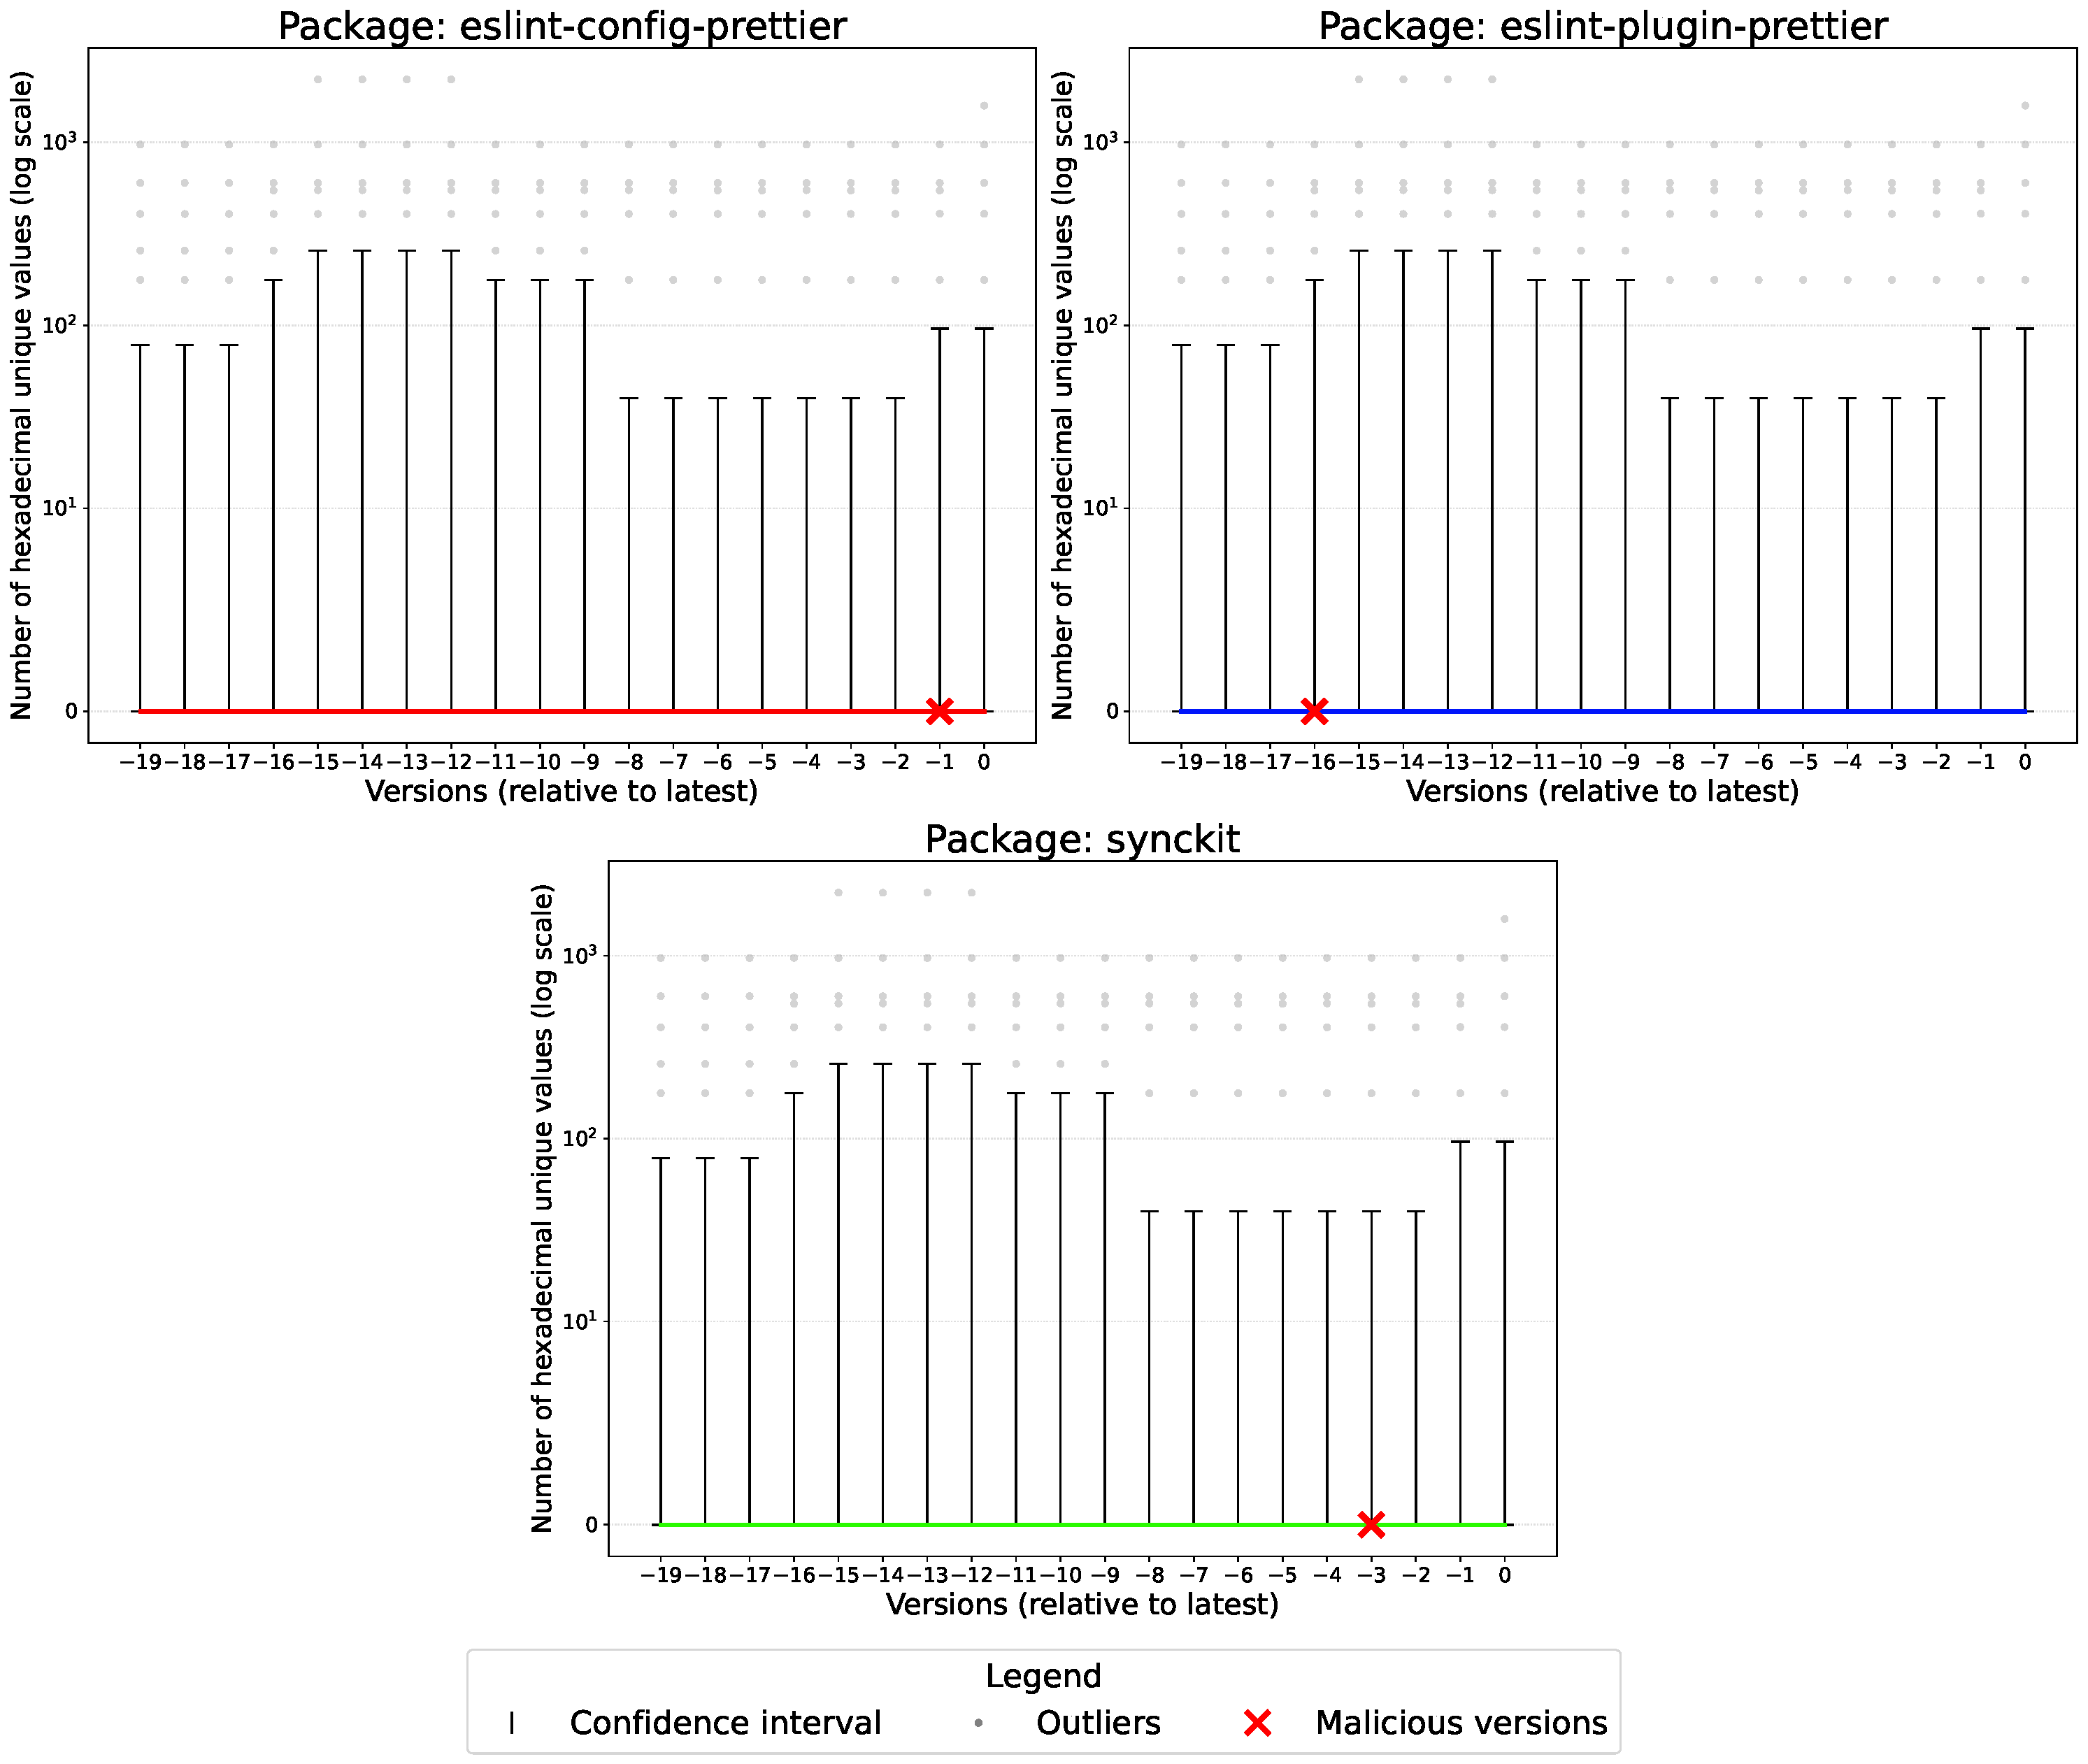
\includegraphics[width=0.97\textwidth]{metrics/hex/hex_plot2singlesingle_AttackA.pdf}
    \caption{Unique Hexadecimal Values Metric: Malware Comparison for Attack~A.}
    \label{fig:fig2HexAttackA}
\end{figure}

In summary, the \emph{Unique Hexadecimal Values} metric is effective for attacks that use hexadecimal encoding as an obfuscation strategy (Attacks~B and~D),
with detection strength scaling with the amount of encoded content, 
as Attack~B produces 455 values, sufficient to cross the outlier boundary,
while Attack~D produces 122,535, an extreme anomaly with no parallel in the goodware baseline.
It is not indicative for Attack~A, whose malicious payload is binary,
nor for Attack~C, where the injected code is clear-text and does not rely on obfuscation.

\begin{figure}[htb]
    \centering
    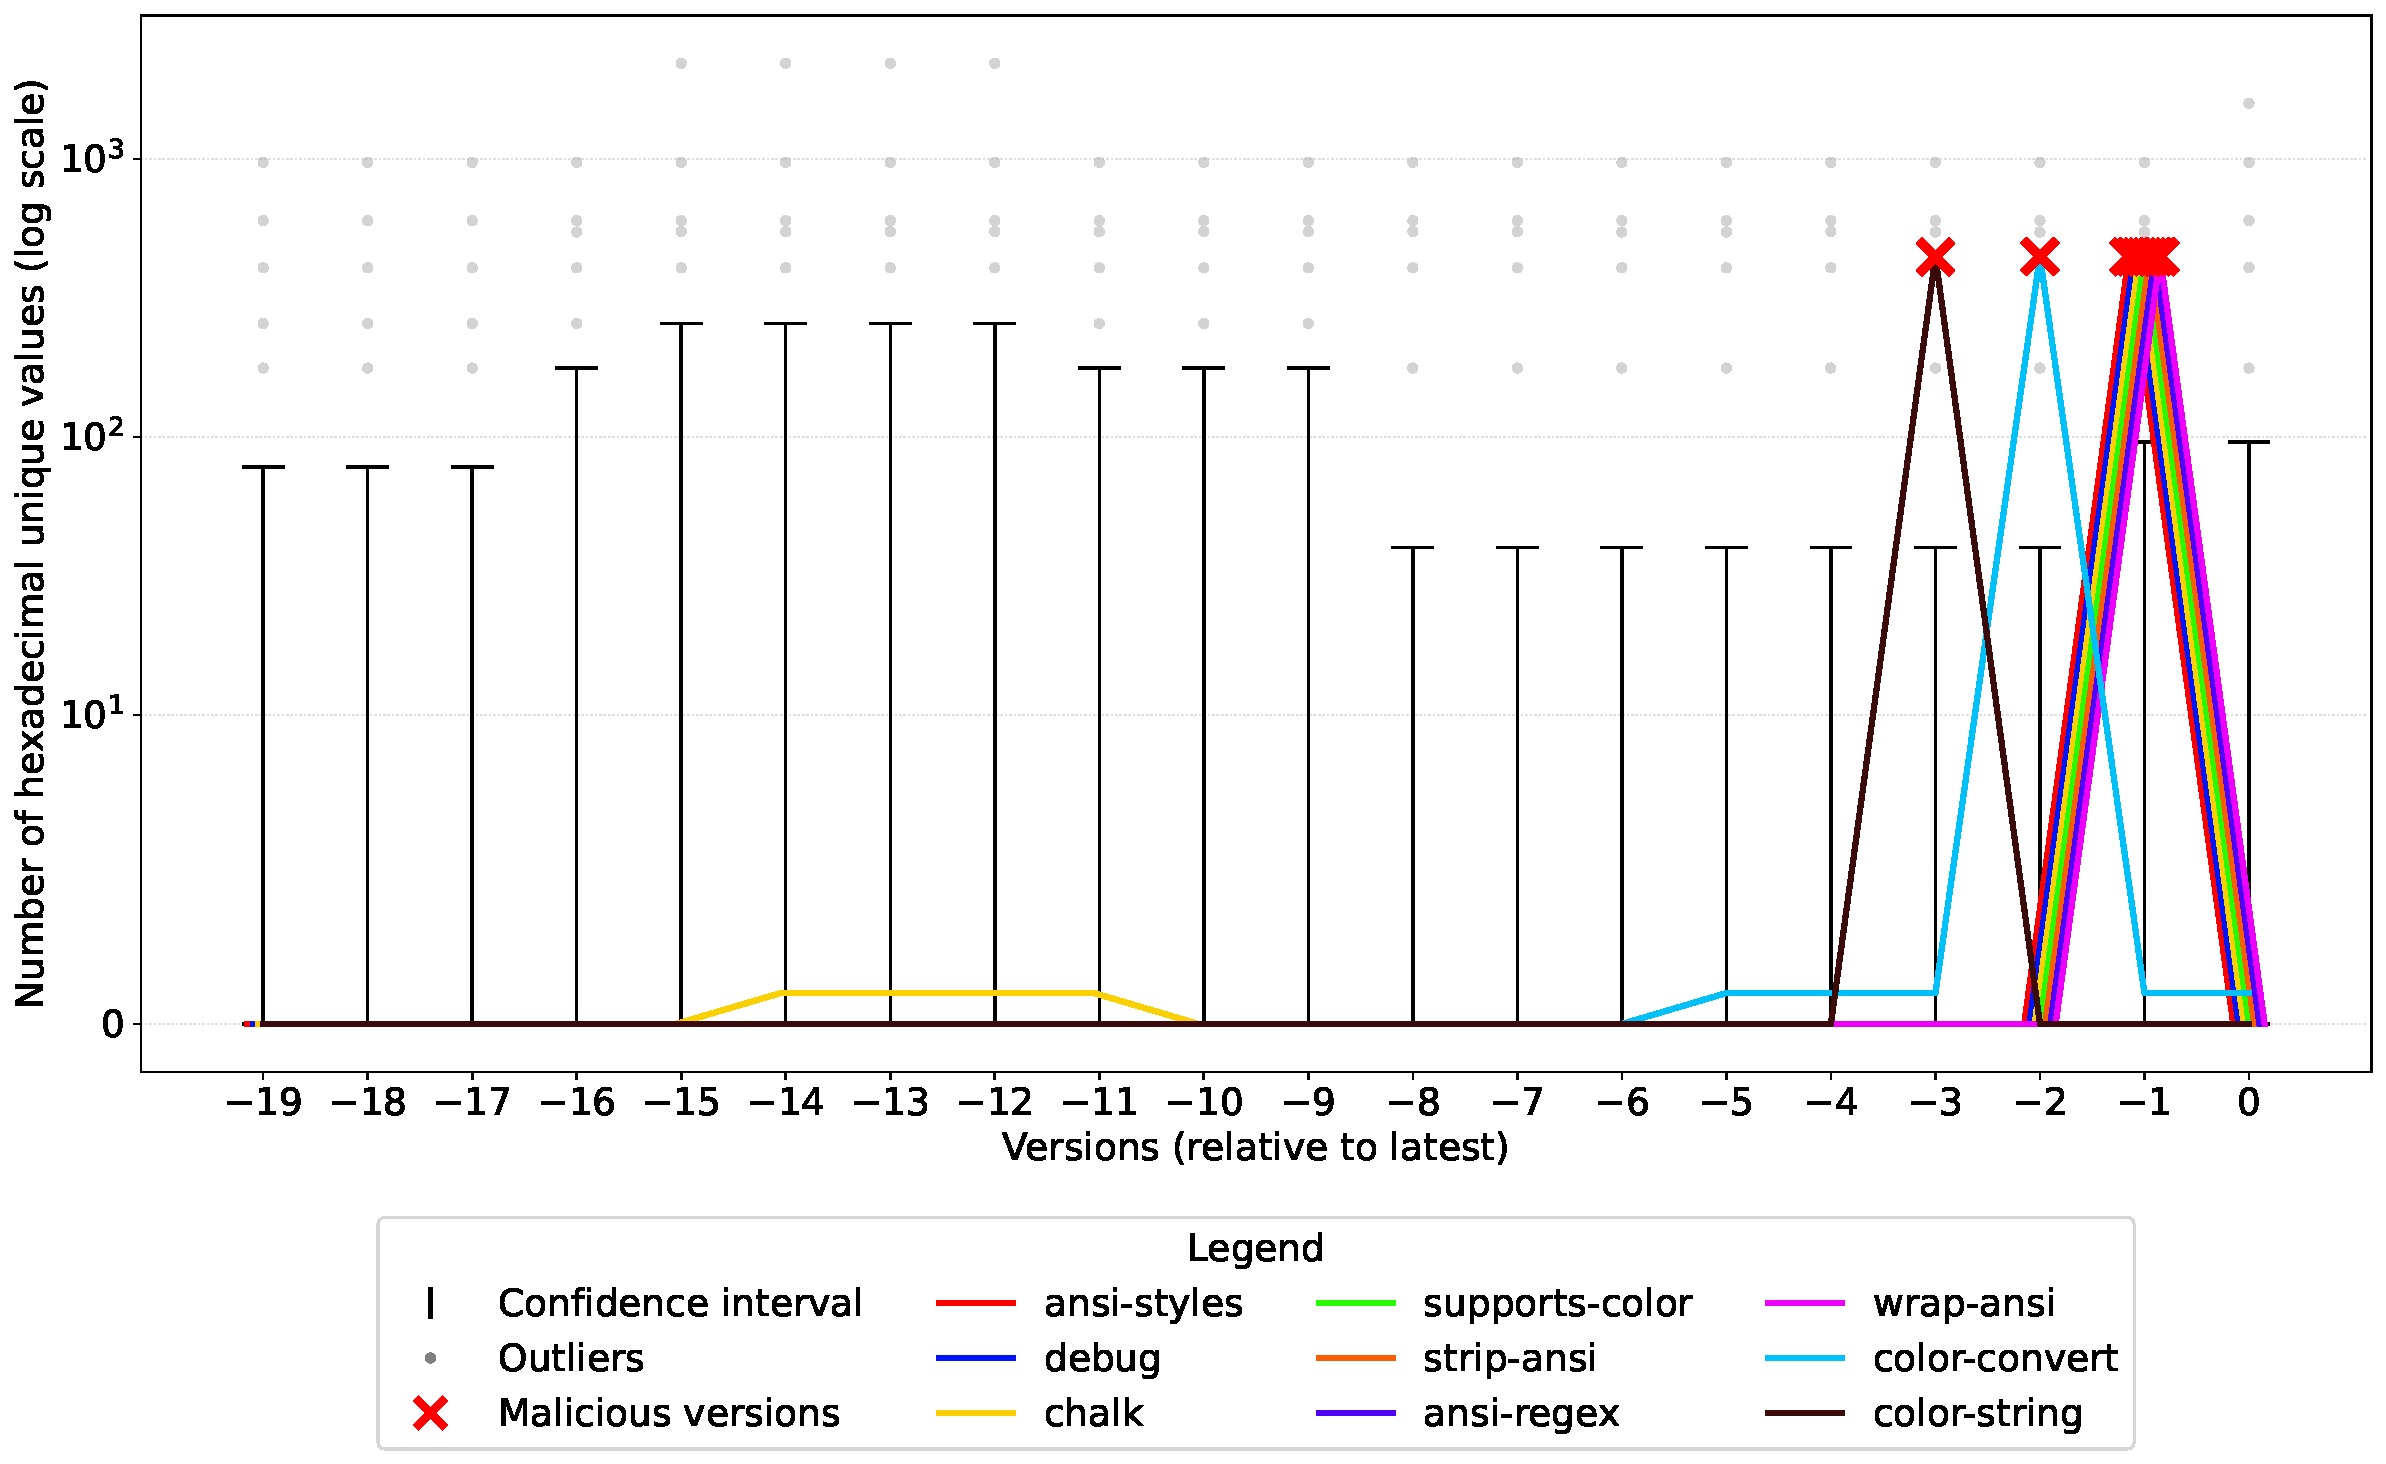
\includegraphics[width=\textwidth]{metrics/hex/hex_plot2single_AttackB.pdf}
    \caption{Unique Hexadecimal Values Metric: Malware Comparison for Attack~B.}
    \label{fig:fig2HexAttackB}
\end{figure}

\begin{figure}[htbp]
    \centering
    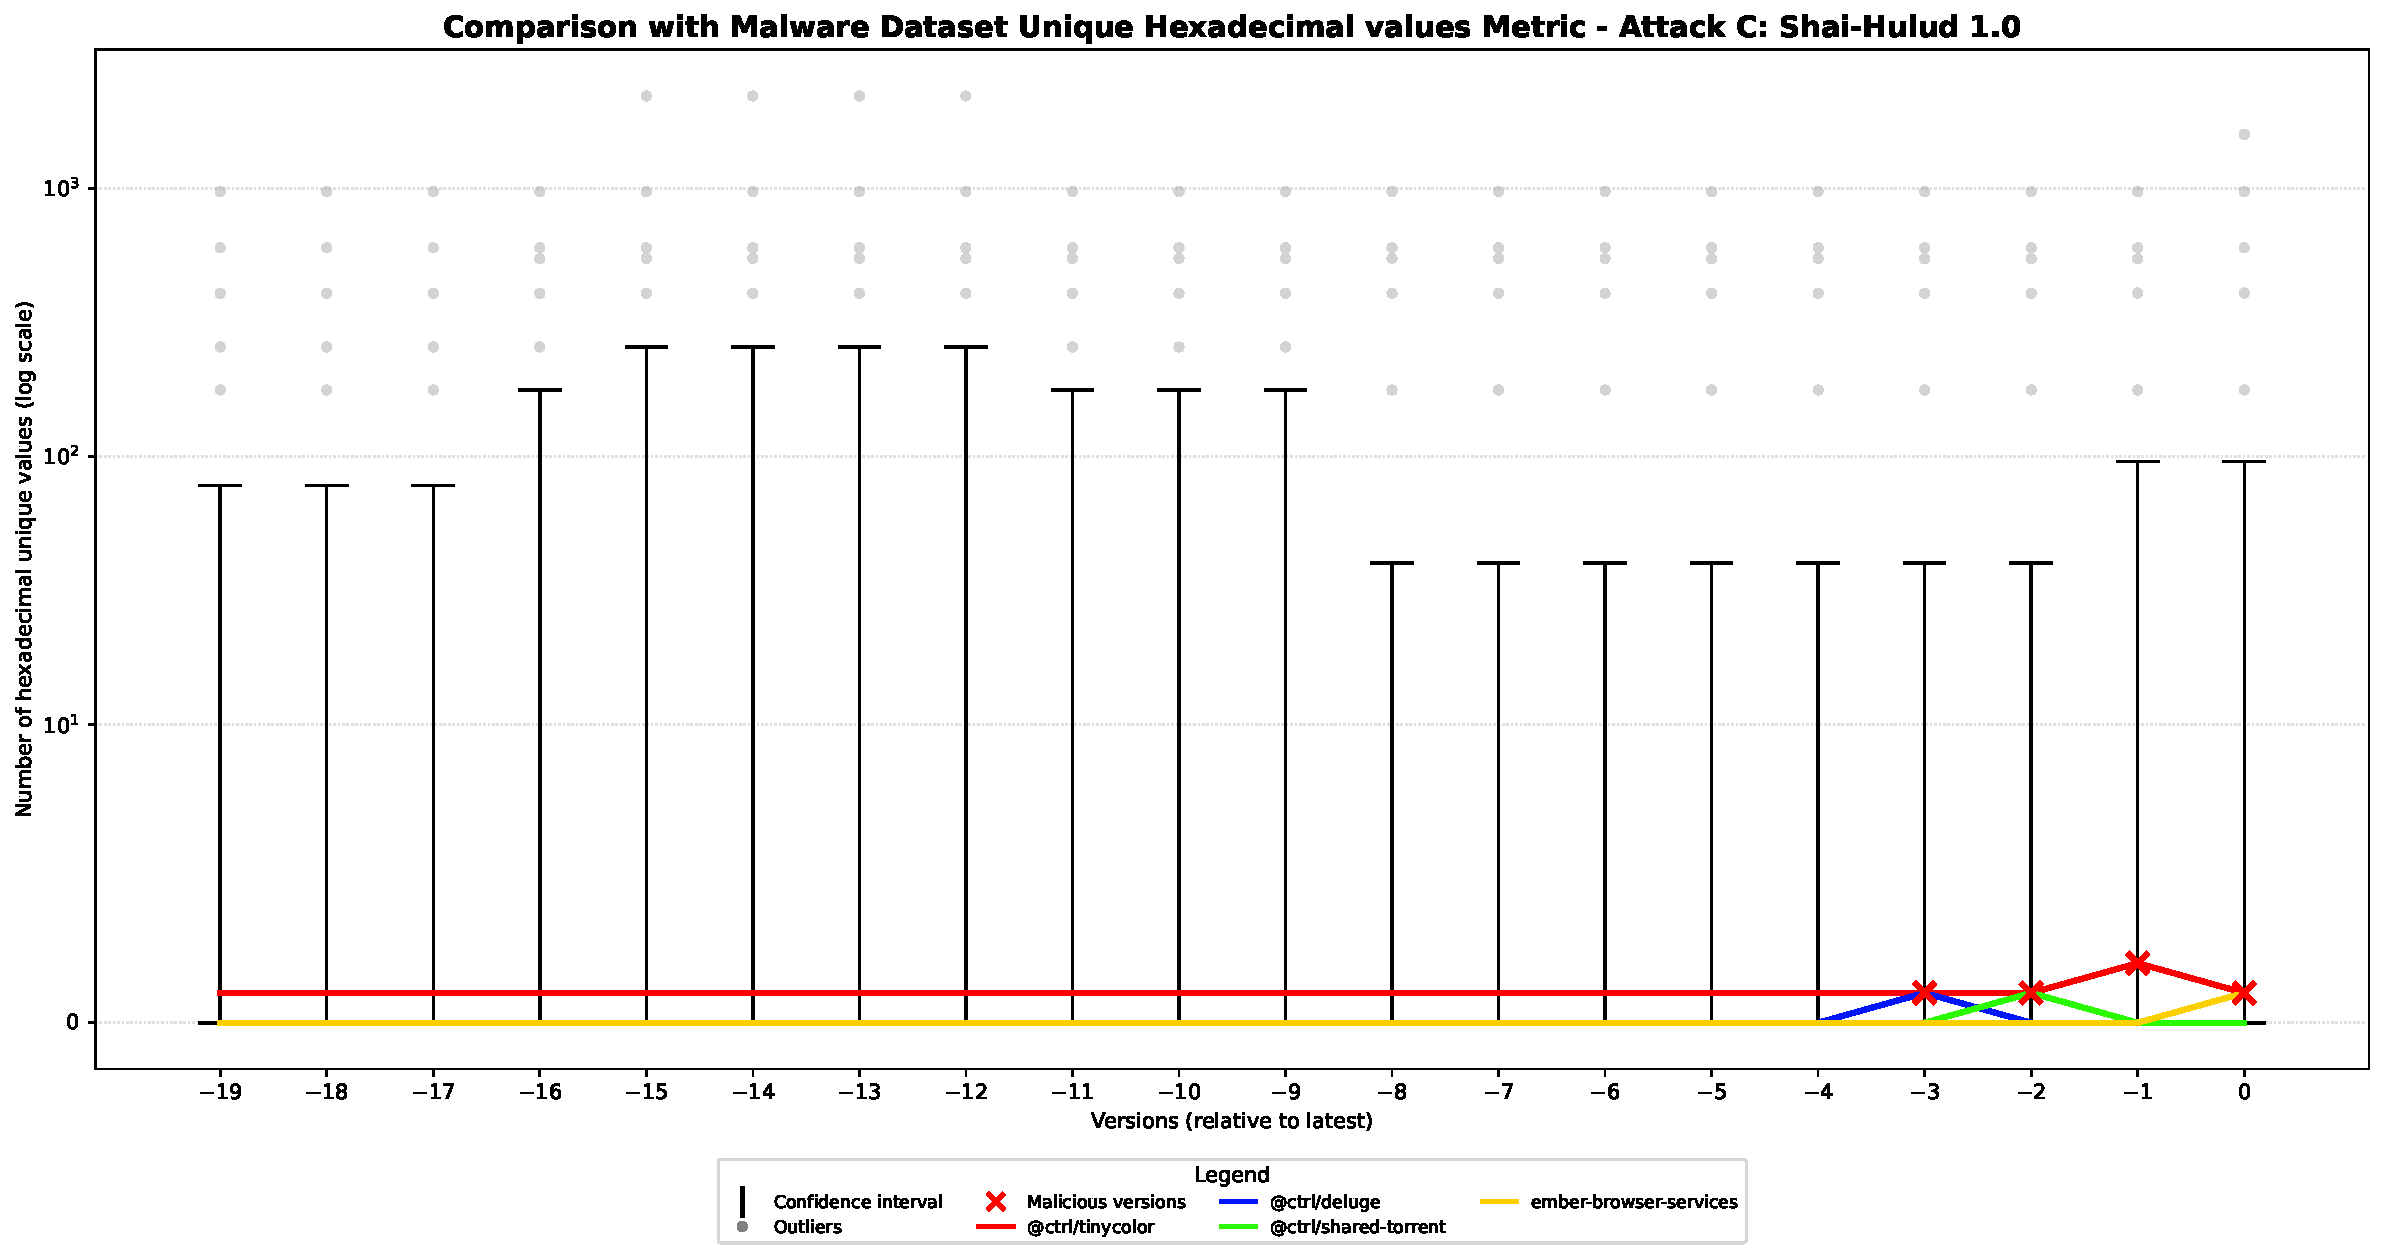
\includegraphics[width=0.90\textwidth]{metrics/hex/hex_plot2single_AttackC.pdf}
    \caption{Unique Hexadecimal Values Metric: Malware Comparison for Attack~C.}
    \label{fig:fig2HexAttackC}

    \vspace{0.3cm} % Spazio verticale tra i due grafici

    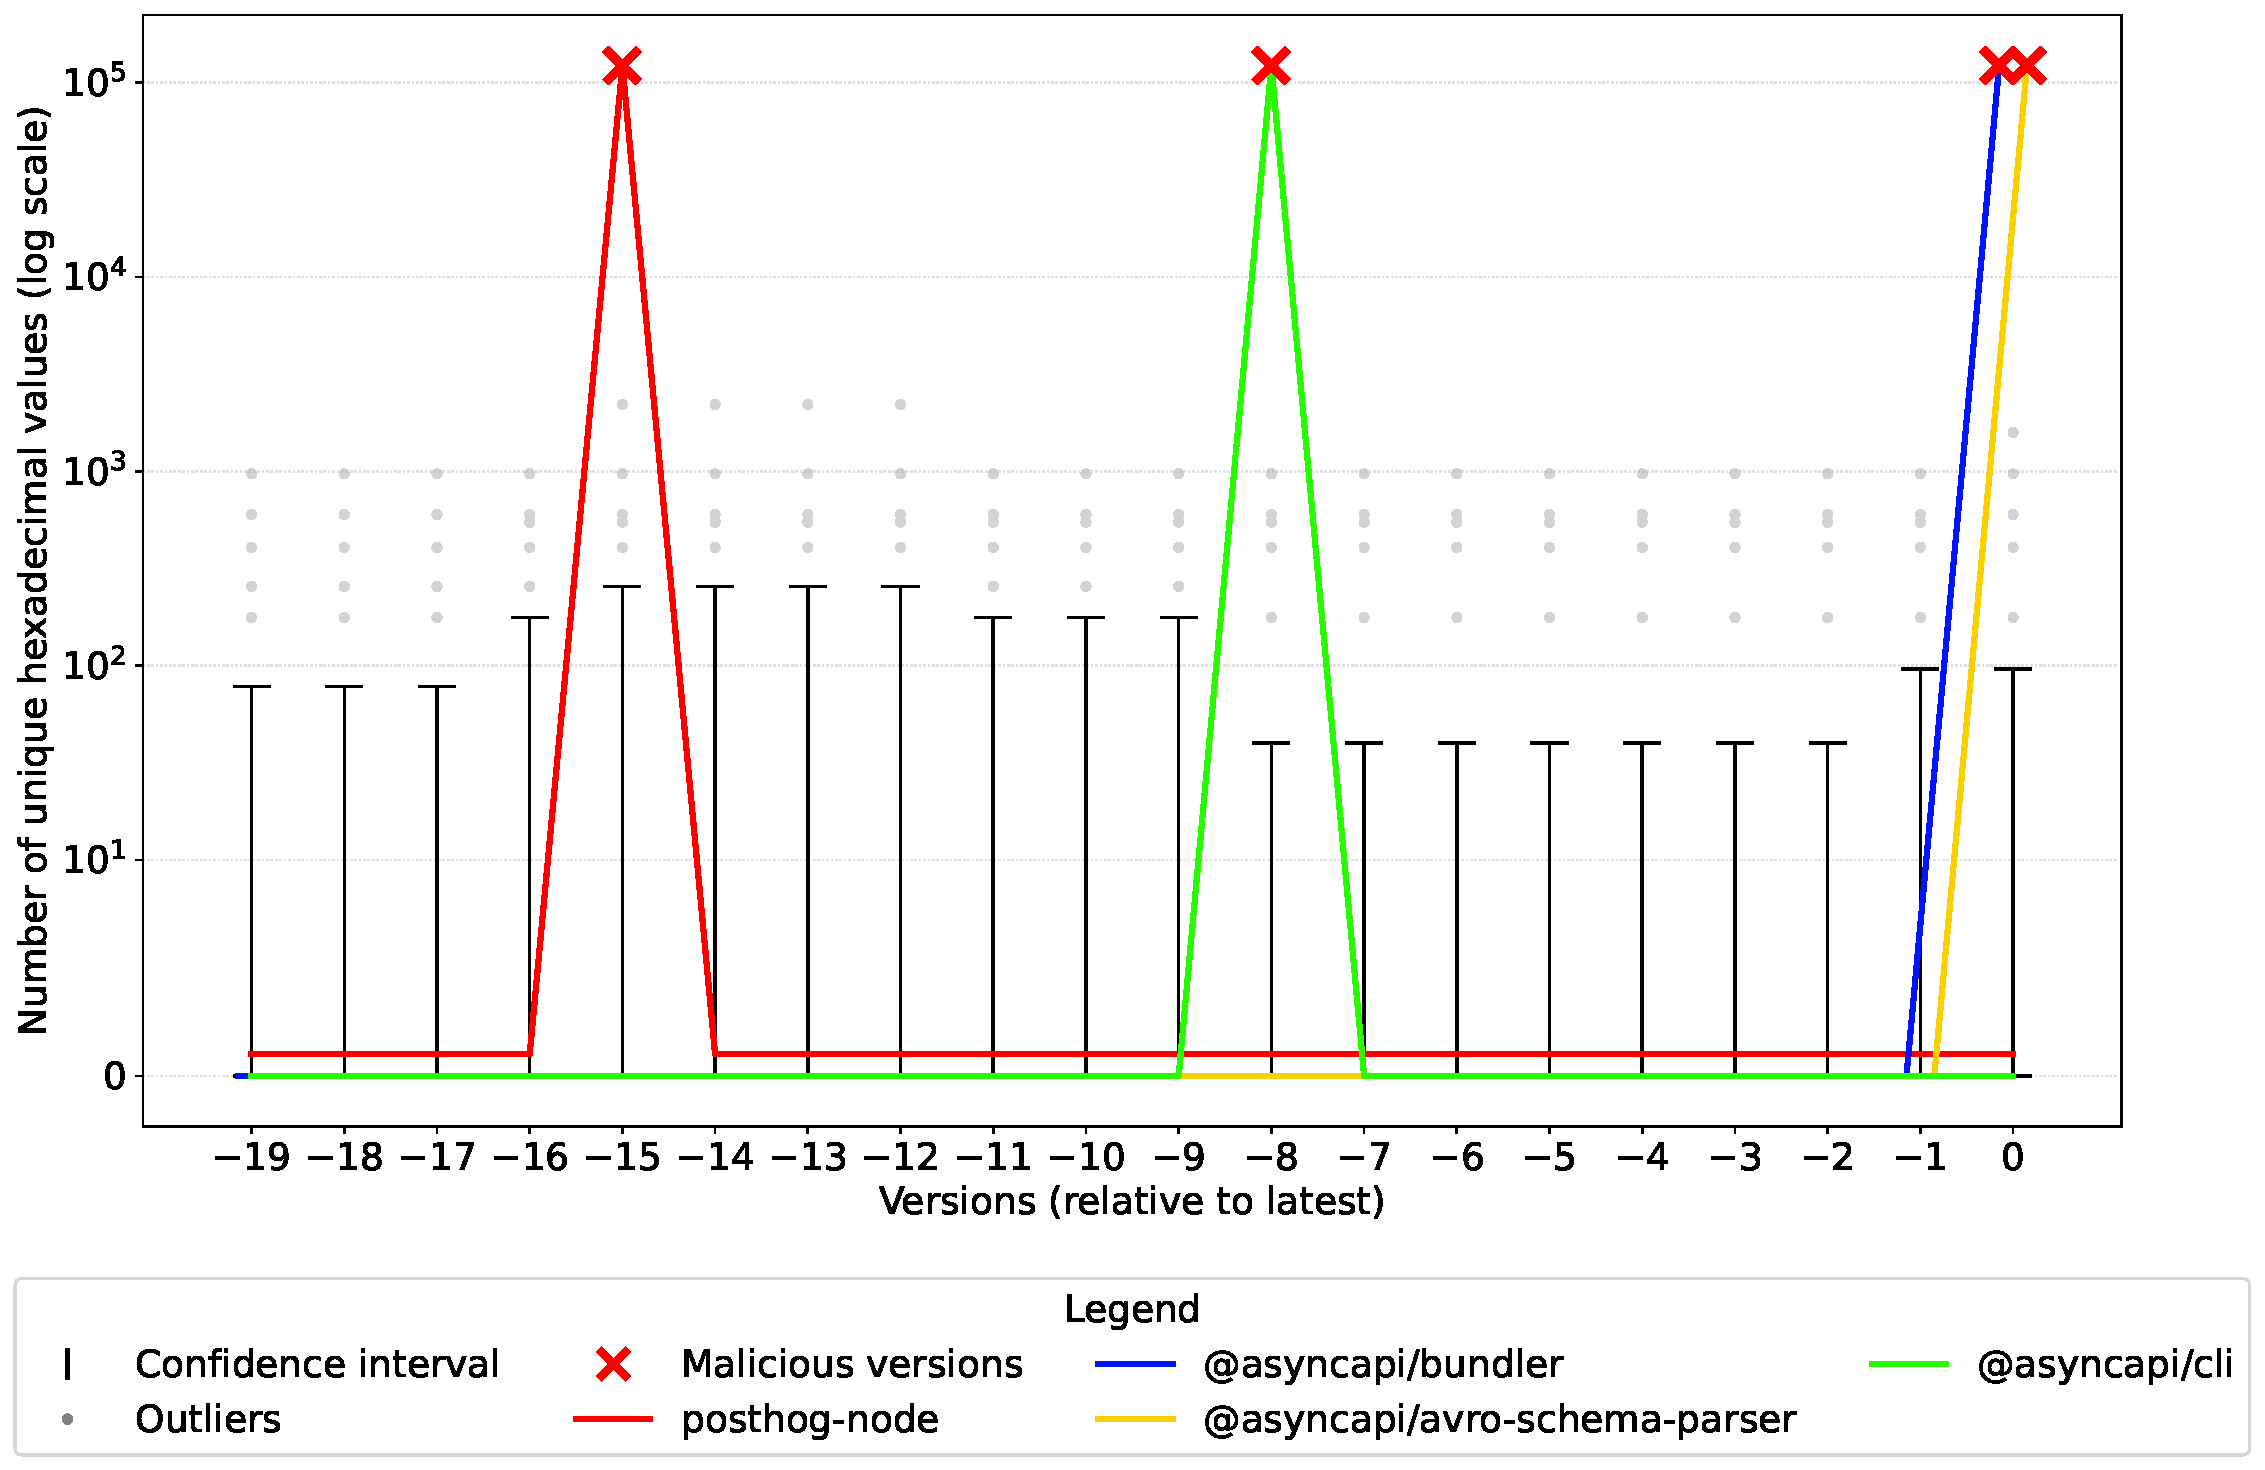
\includegraphics[width=0.90\textwidth]{metrics/hex/hex_plot2single_AttackD.pdf}
    \caption{Unique Hexadecimal Values Metric: Malware Comparison for Attack~D.}
    \label{fig:fig2HexAttackD}
\end{figure}